\section{Clasificador}

\note{Una vez que estamos en contexto con el área, procedemos a hablar de la implementación del clasificador.}

\subsection{Metodología}
\begin{frame}
    \frametitle{Metodología}

    \begin{itemize}
        \item Se utilizan SVM, kNN, DT, GNB y MNB\@.
        \item Se divide en 80\% entrenamiento y 20\% evaluación.
        \item Se usa validación cruzada sobre el conjunto de entrenamiento para resultados intermedios durante el desarollo y el conjunto de evaluación para el resultado final.
    \end{itemize}
\end{frame}

\note{Primero hablamos de la metodología que usamos. Se utilizan las técnicas, SVM, Vecinos más cercanos, Árboles de decisión y dos tipos de clasificadores Naïve Bayes: uno que supone que las probabilidades siguen una distribución gaussiana y otro que supone que siguen una distribución multinomial.

Dividimos el corpus en 80\% entrenamiento y 20\% evaluación. El corpus de evaluación lo dejamos para el final de manera de intentar no sesgarse demasiado a los resultados y que las métricas no sean mentirosas. Mientras se desarrollan las características y el clasificador se utiliza una técnica llamada validación cruzada para evaluar al clasificador. Cuando se quieren estudiar casos puntuales de error, como por ejemplo tweets falsos positivos, se ha partido nuevamente al conjunto de entrenamiento en entrenamiento y evaluación.}

\subsection{Línea base}
\begin{frame}
    \frametitle{Línea base}

    \begin{enumerate}
        \item BoW + MNB

        \item Clasificador que predice según lo que dice la mayoría (Negativo)
    \end{enumerate}

    \begin{center}
        \scriptsize
        \begin{tabular}{ c r r r r r r r }
            & \multicolumn{1}{c}{Precisión} & \multicolumn{1}{c}{Recall} & \multicolumn{1}{c}{$F_1$} & \multicolumn{1}{c}{Prec.\ neg.} & \multicolumn{1}{c}{Rec.\ neg.} & \multicolumn{1}{c}{$F_1$ neg.} & \multicolumn{1}{c}{Acierto} \\
            \midrule
            LB1 & \textbf{65,2} & \textbf{82,7} & \textbf{72,9} & \textbf{96,3} & 91,2 & \textbf{93,7} & \textbf{89,7} \\
            \midrule
            LB2 & N/A & 0,0 & N/A & 82,5 & \textbf{100,0} & 90,4 & 82,5 \\
        \end{tabular}
    \end{center}
\end{frame}

\note{Decidimos establecer una línea base para comparar contra las técnicas utilizadas.

El primero de ellos es un modelo llamado Bag of Words, o bolsa de palabras. La idea es transformar cada tweet en un vector de conteos de las palabras que aparecen. Es decir, las características son cada una de las palabras que aparecen en los tweets. Un tweet por ejemplo puede tener la palabra ``mesa'' 2 veces, la palabra ``arte'' una vez y la palabra ``plato'' ninguna vez. Se combina esto con un clasificador Naïve Bayes multinomial.

El segundo es un clasificador mucho más simple. Se limita a predecir en base a la categoría que fue más frecuente en la etapa de entrenamiento. Dice lo que dice la mayoría, en otras palabras. En este caso dice que todo es negativo, No humor, porque observó al rededor de 83\% de negativos al entrenar.}

\note{Acá se muestran los números que se obtuvieron, en donde tenemos la Precisión [señalar], Recall, F1, lo mismo para los negativos y finalmente el acierto. Se puede observar que la primera línea base supera ampliamente a la segunda.}

\subsection{Características}

\begin{frame}
    \frametitle{Características}

    Qué se busca:

    \begin{itemize}
        \item Contradicción y negatividad
        \item Formato
        \item Informalidad
        \item Orientación en personas
        \item Temas recurrentes en chistes
    \end{itemize}
\end{frame}

\note{Ahora vamos a hablar de las características implementadas. Básicamente buscamos las siguientes cosas: contradicción y negatividad en los tweets, determinado tipo de formato sintáctico, informalidad, que estén centrados en personas y temas recurrentes en chistes.}

\begin{frame}
    \frametitle{Contradicción y negatividad}
    \framesubtitle{Antónimos}

    \begin{itemize}
        \item Se utiliza WordNet
        \item Cantidad de pares de antónimos en el tweet:
    \end{itemize}

    \begin{center}
        \[
            Antonimos(tweet) = \frac{|\{pares\ de\ antonimos\}|}{\sqrt{|tweet|}}
        \]
    \end{center}
\end{frame}

\note{Buscando contradicción realizamos la característica Antónimos. Se cuenta la cantidad de pares de antónimos en el tweet en relación a su largo.}

\begin{frame}
    \frametitle{Contradicción y negatividad}
    \framesubtitle{Negación}

    \begin{itemize}
        \item Cantidad de ``no'' en el tweet
    \end{itemize}
\end{frame}

\note{Se hace también la característica Negación. Se cuenta la cantidad de ``no'' en el tweet.}

\begin{frame}
    \frametitle{Formato}
    \framesubtitle{Diálogo}

    \begin{itemize}
        \item Si el tweet es un diálogo o no
    \end{itemize}
\end{frame}

\note{En cuanto al Formato tenemos primero a Diálogo. Indica si el tweet es un diálogo o no.}

\begin{frame}
    \frametitle{Formato}
    \framesubtitle{Links}

    \begin{itemize}
        \item Cantidad de hipervínculos en el tweet
    \end{itemize}
\end{frame}

\note{Luego sigue Links, que cuenta la cantidad de enlaces en el tweet. Como el humor que buscamos debe ser expresado completamente en textos no tendría sentido un enlace a una imagen por ejemplo.}

\begin{frame}
    \frametitle{Formato}
    \framesubtitle{Preguntas-respuestas}

    \begin{itemize}
        \item Cantidad de preguntas seguidas de respuestas en el tweet.
    \end{itemize}
\end{frame}

\note{Preguntas-respuestas: se cuenta la cantidad de preguntas seguidas de respuestas que hay en el tweet.}

\begin{frame}
    \frametitle{Informalidad}
    \framesubtitle{Exclamación}

    \begin{itemize}
        \item Cantidad de signos de exclamación:
    \end{itemize}

    \begin{center}
        \[
            Exclamacion(tweet) = \frac{|\{signos\ de\ exclamacion\}|}{\sqrt{|tweet|}}
        \]
    \end{center}
\end{frame}

\note{Mirando la Informalidad tenemos por un lado la Exclamación. Cuenta la cantidad de signos de exclamación en relación al largo del tweet. Suele indicar informalidad y potencialmente humor.}

\begin{frame}
    \frametitle{Informalidad}
    \framesubtitle{Hashtags}

    \begin{itemize}
        \item Cantidad de hashtags en el tweet
    \end{itemize}
\end{frame}

\note{Hashtags: cuenta la cantidad de hashtags en el tweet.}

\begin{frame}
    \frametitle{Informalidad}
    \framesubtitle{Palabras fuera del vocabluario (OOV)}

    \begin{itemize}
        \item Cantidad de palabras fuera del vocabulario, dividido entre el total

        \item Son varias características:

        \begin{itemize}
            \item Freeling
            \item Freeling-Google
            \item Freeling-Wiktionary
            \item Wiktionary
        \end{itemize}
    \end{itemize}
\end{frame}

\note{
    Luego sigue OOV\@. Son cuatro características que cuentan la cantidad de palabras fuera del vocabulario en relación al largo del tweet.

    Las distintas combinaciones de diccionarios es debido a ventajas y desventajas de cada uno. \textbf{Freeling} es una herramienta que posee el diccionario más barato de usar que tenemos, porque es offline. Tiene un español más clásico, pero no tiene palabras ``nuevas''. \textbf{Wiktionary} tiene un término medio de todo. Es online, pero no limita su uso, y además tiene algunas palabras modernas. Con \textbf{Google} se pueden obtener muchas palabras ``nuevas'' (como iPhone) y también detección de errores ortográficos, pero limita su uso.
}

\begin{frame}
    \frametitle{Informalidad}
    \framesubtitle{Palabras mayúsculas}

    \begin{itemize}
        \item Cantidad de palabras totalmente en mayúsculas:
    \end{itemize}

    \begin{center}
        \[
            PalabrasMayusculas(tweet) = \frac{|\{palabras\ mayusculas\}|}{\sqrt{|tweet|}}
        \]
    \end{center}
\end{frame}

\note{Palabras mayúsculas: se cuenta la cantidad de palabras totalmente en mayúsculas en relación a la cantidad de palabras del tweet. Cuando hay palabras en mayúsculas es como si estuvieran gritando en el tweet, lo cual da informalidad y potencialmente humor, ya que creemos que el humor suele ser informal.}

\begin{frame}
    \frametitle{Informalidad}
    \framesubtitle{Palabras no españolas}

    \begin{itemize}
        \item Cantidad de palabras que tienen caracteres fuera del alfabeto español, normalizado según el total.
    \end{itemize}
\end{frame}

\note{Palabras no españolas: se cuenta la cantidad de palabras que contienen caracteres fuera del alfabeto español, normalizando según el total. Se fija por la presencia de caracteres raros que indican, de vuelta, informalidad.}

\begin{frame}
    \frametitle{Orientación en personas}
    \framesubtitle{Primera y segunda persona}

    \begin{itemize}
        \item Se busca por palabras flexionadas en primera persona y se hace lo mismo con segunda persona
    \end{itemize}
\end{frame}

\note{En cuanto a Orientación en personas tenemos Primera persona y Segunda persona, dos características. La primera busca palabras en primera persona, ya sean verbos, sustantivos, adjetivos; como ``hago'' o ``yo''. La segunda busca palabras como ``tú'' o ``haces''.}

\begin{frame}
    \frametitle{Temas recurrentes en chistes}
    \framesubtitle{Distancia temática}

    \begin{itemize}
        \item Cercanía a una categoría de chiste de Chistes.com o cercanía a una oración de Wikipedia.

        \item BoW + MNB

        \item Categorías:

        \begin{itemize}
            \item Chistes cortos
            \item Adivinanzas
            \item Animales
            \item Atlantes
            \item Otros\ldots
        \end{itemize}
    \end{itemize}
\end{frame}

\note{En Temas recurrentes en chistes tenemos primero Distancia temática. La idea es fijarse qué cercanía tiene un tweet a una categoría de chistes de la página Chistes.com, contrastando con oraciones de Wikipedia. Se toman las 5 categorías que más tienen chistes, armando 5 características entonces. Cada una arma un subclasificador, utilizando el modelo Bag of Words con Naïve Bayes multinomial, así como la primera línea base, tomando como características a los conteos de cada palabra. Se obtiene entonces una categoría (chiste de Chistes.com u oración de Wikipedia) y a la vez un número que indica la probabilidad de acercarse a una categoría, que es particularmente devuelto por Naïve Bayes.}

\begin{frame}
    \frametitle{Temas recurrentes en chistes}
    \framesubtitle{Jerga sexual}

    \begin{itemize}
        \item Se arma un diccionario de jerga sexual mediante \emph{Bootstrapping} en Twitter.

        \item Intersección de multiconjuntos:
    \end{itemize}

    \begin{center}
        \[
            JergaSexual(tweet) = \frac{|tweet \cap DIC_{JS}|}{\sqrt{|tweet|}}
        \]
    \end{center}
\end{frame}

\note{Jerga sexual. Se arma un diccionario de jerga sexual. Primero intuitivamente. Luego se refuerza mediante una técnica, llamada Bootstrapping, en la que se buscan tweets que aparezcan las palabras de este primer diccionario y nos fijamos qué palabras más co-ocurren con ellas, agrandando el diccionario.

Luego nos fijamos la cantidad de palabras de los tweets que pertenecen a este diccionario, en relación al total de palabras del tweet.}

\begin{frame}
    \frametitle{Temas recurrentes en chistes}
    \framesubtitle{Palabras clave}

    \begin{itemize}
        \item Lista de palabras frecuentes en chistes
        \item Intersección de multiconjuntos:
    \end{itemize}

    \begin{center}
        \[
            PalabrasClave(tweet) = \frac{|tweet \cap DIC_{PF}|}{\sqrt{|tweet|}}
        \]
    \end{center}
\end{frame}

\note{En Palabras clave se arma un diccionario de palabras comunes en chistes empíricamente, como ``mamá'' y ``Jaimito'', y luego se procede de manera similar a la característica anterior con el diccionario.}

\begin{frame}
    \frametitle{Temas recurrentes en chistes}
    \framesubtitle{Presencia de animales}

    \begin{itemize}
        \item Se conforma una lista de animales a partir de los chistes de animales de Chistes.com ($DIC_A$)

        \item Intersección de multiconjuntos:

        \begin{center}
            \[
                PresenciaAnimales(tweet) = \frac{|tweet \cap DIC_A|}{\sqrt{|tweet|}}
            \]
        \end{center}
    \end{itemize}
\end{frame}

\note{Se conforma una lista de animales a partir de las palabras que aparecen en los chistes de animales de Chistes.com. Luego se procede como antes, contando la ocurrencia de palabras de un tweet en el diccionario y normalizando según la cantidad de palabras del tweet.}

\subsection{Selección de características}
\begin{frame}[allowframebreaks]
    \frametitle{Selección de características}

    \begin{itemize}
        \item ExtraTrees es usado para hacer un ranking de características.

        \item Se utiliza la Eliminación recursiva de atributos para seleccionar aquellos relevantes y no redundantes.
    \end{itemize}

    \note{Luego se procede a seleccionar las características. La idea es quitar aquellas irrelevantes o redundantes. Se procede primero utilizando una técnica llamada ExtraTrees, que genera una cantidad fija de Árboles de decisión aleatorios, y se fija qué características discriminan mejor. Se utiliza para hacer un ranking de las características.

    Luego se utiliza la Eliminación recursiva de atributos para seleccionar finalmente las características. La técnica procede a quitar las características más irrelevantes una a una y fijarse con qué número se obtiene mejor acierto.}

    \framebreak{}

    ExtraTrees:

    \begin{center}
        \tiny
        \begin{tabular}{ c r }
            \multicolumn{1}{c}{\textbf{Característica}} & \multicolumn{1}{c}{\textbf{Valor}} \\
            CLASE & 74,05 \\
            Diálogo & 10,86 \\
            Distancia temática: Otros\ldots & 03,07 \\
            Distancia temática: Atlantes & 02,65 \\
            Distancia temática: Chistes cortos & 02,53 \\
            Preguntas-respuestas & 01,98 \\
            Distancia temática: Adivinanzas & 0,95 \\
            Distancia temática: Animales & 0,87 \\
            Palabras clave & 0,57 \\
            Exclamación & 0,57 \\
            Hashtags & 0,55 \\
            Links & 0,54 \\
            Primera persona & 0,21 \\
            Segunda persona & 0,15 \\
            OOV Freeling & 0,08 \\
            Palabras mayúsculas & 0,06 \\
            ALEATORIA & 0,06 \\
            Jerga sexual & 0,06 \\
            Negación & 0,05 \\
            OOV Wiktionary & 0,04 \\
            OOV Freeling Wiktionary & 0,03 \\
            Presencia de animales & 0,03 \\
            OOV Freeling Google & 0,03 \\
            Antónimos & 0,02 \\
            Palabras no españolas & 0,00 \\
        \end{tabular}
    \end{center}

    \note{Se obtiene esta tabla. Se introducen dos características ficticias para comparar. La primera es CLASE, una característica que sabe exactamente si un tweet es humorístico o no, sabe la solución. Por otro lado está ALEATORIA, que tiene un valor aleatorio.

    Observar que por ejemplo Diálogo, Preguntas-respuestas y las de Distancia temática son las características que más discriminan al humor. Ver por otro lado que características como las de OOV, Antónimos y Jerga sexual resultan ser peores que el azar.}

    \framebreak{}

    Eliminación recursiva de atributos:

    \begin{center}
        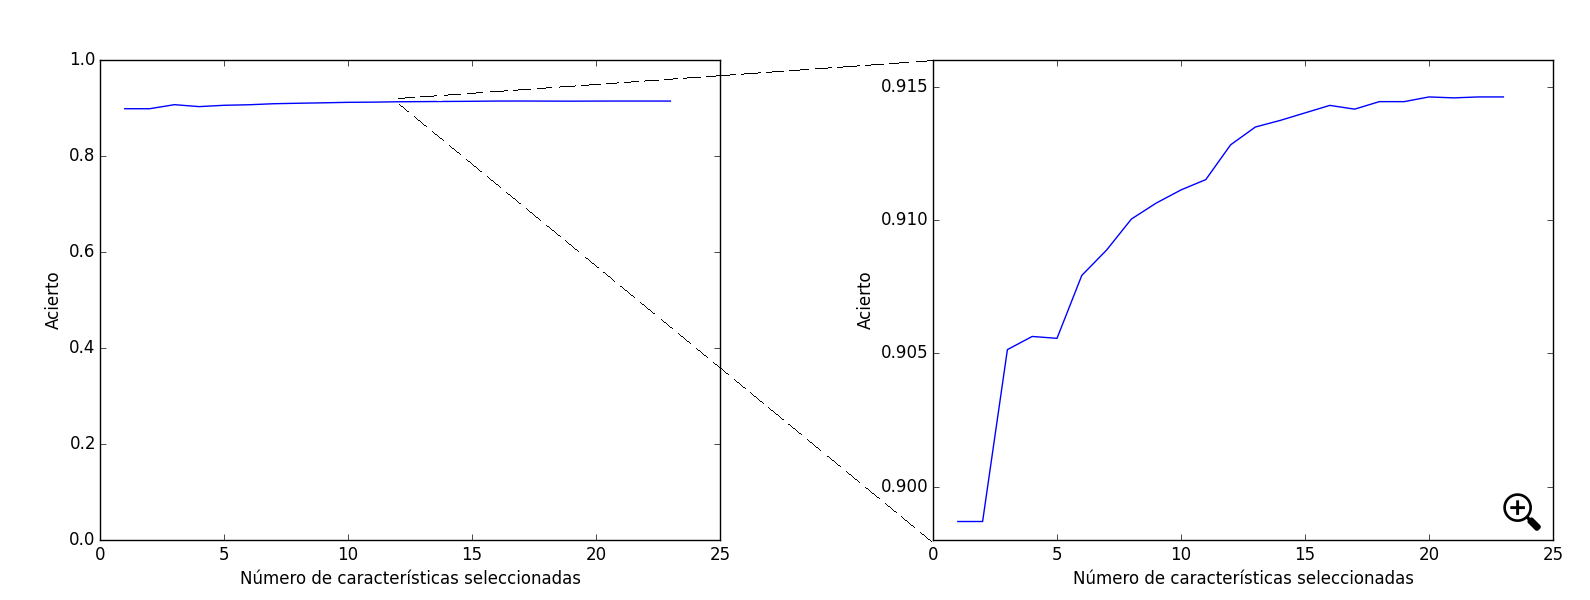
\includegraphics[height=4cm]{rfe.png}

        \vspace{1cm}

        Se descartan Negación, Palabras no españolas y Antónimos
    \end{center}
\end{frame}

\note{Esta es la gráfica resultado que se obtiene de la Eliminación recursiva de atributos. El máximo acierto se obtiene al eliminar tres, pero observar que la variación total del acierto es muy poca, inclusive para el máximo.

Finalmente se descartan entonces Negación, Palabras no españolas y Antónimos.

A continuación mi compañero Matías va a proceder a mostrar los resultados obtenidos.}

\subsection{Resultados obtenidos}
\begin{frame}
    \frametitle{Resultados obtenidos}

    \begin{center}
        \scriptsize
        \begin{tabular}{ c r r r r r r r }
            & \multicolumn{1}{c}{Precisión} & \multicolumn{1}{c}{Recall} & \multicolumn{1}{c}{$F_1$} & \multicolumn{1}{c}{Prec.\ neg.} & \multicolumn{1}{c}{Rec.\ neg.} & \multicolumn{1}{c}{$F_1$ neg.} & \multicolumn{1}{c}{Acierto} \\
            \midrule
            LB1 & \textbf{61,7} & \textbf{84,6} & \textbf{71,4} & \textbf{96,6} & 89,2 & 71,4 & \textbf{88,5} \\
            \midrule
            LB2 & N/A & 0,0 & N/A & 83,0 & \textbf{100,0} & \textbf{90,7} & 83,0 \\
            \midrule
            \midrule
            SVM & 83,6 & 68,9 & \textbf{75,5} & 93,8 & 97,2 & \textbf{95,5} & \textbf{92,5} \\
            \midrule
            DT & 66,5 & 67,5 & 67,0 & 93,3 & 93,0 & 93,2 & 88,9 \\
            \midrule
            GNB & 57,5 & \textbf{78,2} & 66,3 & \textbf{95,2} & 88,2 & 91,5 & 86,5 \\
            \midrule
            MNB & \textbf{84,8} & 60,0 & 70,3 & 92,3 & \textbf{97,8} & 95,0 & 91,4 \\
            \midrule
            KNN & 81,3 & 66,3 & 73,0 & 93,4 & 96,9 & 95,1 & 91,7 \\
        \end{tabular}

        \begin{center}
            Mejor técnica: \textbf{SVM}
        \end{center}

        \begin{tabular}{ c r r }
            \textbf{son/clasif.} & Positivos & Negativos \\
            \midrule
            Positivos & 842 & 381 \\
            \midrule
            Negativos & 165 & 5805 \\
        \end{tabular}
    \end{center}
\end{frame}

\subsection{Otros análisis}

\subsubsection{Evaluación en el conjunto de entrenamiento}
\begin{frame}
    \frametitle{Evaluación en el conjunto de entrenamiento}

    \begin{itemize}
        \item Es una ``cota superior''
    \end{itemize}

    \begin{center}
        \scriptsize
        \begin{tabular}{ c r r r r r r r }
            & \multicolumn{1}{c}{Precisión} & \multicolumn{1}{c}{Recall} & \multicolumn{1}{c}{$F_1$} & \multicolumn{1}{c}{Prec.\ neg.} & \multicolumn{1}{c}{Rec.\ neg.} & \multicolumn{1}{c}{$F_1$ neg.} & \multicolumn{1}{c}{Acierto} \\
            \midrule
            SVM & 87,5 & 69,6 & 77,5 & 94,2 & 98,0 & 96,1 & 93,3 \\
            \midrule
            DT & \textbf{100,0} & \textbf{98,8} & \textbf{99,4} & \textbf{99,8} & \textbf{100,0} & \textbf{99,9} & \textbf{99,8} \\
            \midrule
            GNB & 58,1 & 77,7 & 66,4 & 95,2 & 88,8 & 91,9 & 86,9 \\
            \midrule
            MNB & 84,6 & 58,9 & 69,5 & 92,3 & 97,9 & 95,0 & 91,7 \\
            \midrule
            KNN & 87,0 & 71,5 & 78,5 & 94,5 & 97,9 & 96,2 & 93,5 \\
        \end{tabular}
    \end{center}
\end{frame}

\begin{frame}
    \frametitle{Evaluación en el conjunto de entrenamiento II}

    \begin{itemize}
        \item ¿Por qué DT no da 100\%? Debería darlo.
        \item Las características no discriminan completamente a la clase.
        \item ¿Hay errores en el corpus?
    \end{itemize}
\end{frame}

\begin{frame}[allowframebreaks]
    \frametitle{Inconsistencias en el corpus}

    \begin{itemize}
        \item Siguiendo la distancia mínima de edición en tweets (la granularidad es una palabra): se encontraron 367 pares de tweets ``parecidos'' pero con distinto valor de la clase objetivo.
    \end{itemize}

    \begin{example}
        Limpiar tu cuarto = 1\% limpieza. 30\% quejarse. 69\% jugar con lo que vas encontrando.
    \end{example}

    \begin{example}
        Limpiar tu cuarto:

        1\% limpieza.

        30\% quejarse.

        69\% jugar con lo que vas encontrando.
    \end{example}

    \framebreak{}

    \begin{itemize}
        \item Luego se buscan aquellos con mismos valores de atributos pero distinta clase: 30 pares encontrados.
    \end{itemize}

    \begin{example}
        \#TerminarUnaNotaDeSuicidioCon Soy Darks.
    \end{example}

    \begin{example}
        \#SiYoMeLlamaraKevinRoldan Me suicidaria.
    \end{example}
\end{frame}

\begin{frame}
    \frametitle{Inconsistencias en el corpus III}

    \begin{itemize}
        \item Hay inconsistencias en la anotación (era esperado)
        \item Hay una mejora sobre el corpus de entrenamiento, en la ``cota superior'', quitando estas instancias:

        \begin{center}
            \scriptsize
            \begin{tabular}{ c r r r r r r r }
                \textbf{SVM} & \multicolumn{1}{c}{Precisión} & \multicolumn{1}{c}{Recall} & \multicolumn{1}{c}{$F_1$} & \multicolumn{1}{c}{Prec.\ neg.} & \multicolumn{1}{c}{Rec.\ neg.} & \multicolumn{1}{c}{$F_1$ neg.} & \multicolumn{1}{c}{Acierto} \\
                \midrule
                Antes & 87,5 & 69,6 & 77,5 & 94,2 & 98,0 & 96,1 & 93,3 \\
                \midrule
                Después & \textbf{89,0} & \textbf{71,3} & \textbf{79,1} & \textbf{94,7} & \textbf{98,3} & \textbf{96,5} & \textbf{94,0} \\
            \end{tabular}
        \end{center}
    \end{itemize}

    \begin{itemize}
        \item Y en el de corpus de evaluación:

        \begin{center}
            \scriptsize
            \begin{tabular}{ c r r r r r r r }
                \textbf{SVM} & \multicolumn{1}{c}{Precisión} & \multicolumn{1}{c}{Recall} & \multicolumn{1}{c}{$F_1$} & \multicolumn{1}{c}{Prec.\ neg.} & \multicolumn{1}{c}{Rec.\ neg.} & \multicolumn{1}{c}{$F_1$ neg.} & \multicolumn{1}{c}{Acierto} \\
                \midrule
                Antes & 83,6 & 68,9 & 75,5 & 93,8 & 97,2 & 95,5 & 92,5 \\
                \midrule
                Después & \textbf{85,7} & \textbf{69,2} & \textbf{76,6} & \textbf{94,2} & \textbf{97,8} & \textbf{95,9} & \textbf{93,1} \\
            \end{tabular}
        \end{center}
    \end{itemize}
\end{frame}

\subsubsection{Tweets censurados}
\begin{frame}
    \frametitle{Tweets censurados}

    \begin{itemize}
        \item El clasificador está sesgado a no conocer los tweets con contenido explícito
        \item Se anotan a mano los 303 tweets censurados y se agregan
        \item Hay una pequeña mejora:
        \begin{center}
            \scriptsize
            \begin{tabular}{ c r r r r r r r }
                \textbf{SVM} & \multicolumn{1}{c}{Precisión} & \multicolumn{1}{c}{Recall} & \multicolumn{1}{c}{$F_1$} & \multicolumn{1}{c}{Prec.\ neg.} & \multicolumn{1}{c}{Rec.\ neg.} & \multicolumn{1}{c}{$F_1$ neg.} & \multicolumn{1}{c}{Acierto} \\
                \midrule
                Antes & 83,6 & 68,9 & 75,5 & \textbf{93,8} & \textbf{97,2} & \textbf{95,5} & \textbf{92,5} \\
                \midrule
                Después & \textbf{84,0} & \textbf{69,6} & \textbf{76,1} & 93,7 & \textbf{97,2} & 95,4 & 92,3 \\
            \end{tabular}
        \end{center}
        \item Un nuevo estudio de importancia de las características revela que no varía Jerga sexual: se agrega más variedad que jerga sexual.
    \end{itemize}
\end{frame}

\subsubsection{Restricción a cuentas humorísticas}
\begin{frame}
    \frametitle{Restricción a cuentas humorísticas}

    \begin{itemize}
        \item Es una tarea más difícil
        \item Igualmente se logran buenos resultados:

        \begin{center}
            \scriptsize
            \begin{tabular}{ c r r r r r r r }
                & \multicolumn{1}{c}{Precisión} & \multicolumn{1}{c}{Recall} & \multicolumn{1}{c}{$F_1$} & \multicolumn{1}{c}{Prec.\ neg.} & \multicolumn{1}{c}{Rec.\ neg.} & \multicolumn{1}{c}{$F_1$ neg.} & \multicolumn{1}{c}{Acierto} \\
                \midrule
                SVM & \textbf{81,9} & 73,8 & 77,6 & 78,5 & \textbf{85,4} & \textbf{81,8} & \textbf{79,9} \\
                \midrule
                DT & 74,5 & 75,5 & 75,0 & 72,2 & 71,1 & 71,7 & 74,1 \\
                \midrule
                GNB & 78,7 & 78,6 & \textbf{78,6} & 76,1 & 76,3 & 76,2 & 77,5 \\
                \midrule
                MNB & 68,5 & \textbf{85,5} & 76,1 & \textbf{83,3} & 64,6 & 72,9 & 74,6 \\
                \midrule
                KNN & 79,2 & 73,0 & 76,0 & 77,4 & 82,9 & 80,1 & 78,1 \\
            \end{tabular}
        \end{center}
    \end{itemize}
\end{frame}

\subsubsection{Clasificación según categorías de cuentas no humorísticas}
\begin{frame}
    \frametitle{Clasificación según categorías de cuentas no humorísticas}

    \begin{center}
        \scriptsize
        \begin{tabular}{ c r r r r r r r }
            \textbf{SVM} & \multicolumn{1}{c}{Precisión} & \multicolumn{1}{c}{Recall} & \multicolumn{1}{c}{$F_1$} & \multicolumn{1}{c}{Prec.\ neg.} & \multicolumn{1}{c}{Rec.\ neg.} & \multicolumn{1}{c}{$F_1$ neg.} & \multicolumn{1}{c}{Acierto} \\
            \midrule
            Noticias & \textbf{97,0} & \textbf{95,2} & \textbf{96,1} & \textbf{97,0} & \textbf{98,1} & \textbf{97,5} & \textbf{97,0} \\
            \midrule
            Reflexiones & 95,0 & 83,0 & 88,6 & 84,0 & 95,3 & 89,3 & 88,9 \\
            \midrule
            Curiosidades & 94,6 & 83,7 & 88,9 & 88,2 & 96,3 & 92,1 & 90,7 \\
        \end{tabular}
    \end{center}
\end{frame}
